\begin{frame}{Dag-like \only<9->{\alert{real}} communication game for a relation $N: U \times V \to T$}
    Triple $(H, A, B)$, where $H$ is directed acyclic graph, $A: H \times U \to \only<-8>{\{0, 1\}}
    \only<9->{\alert{\mathbb{R}}}$~and $B: H \times V \to \only<-8>{\{0, 1\}}
    \only<9->{\alert{\mathbb{R}}}$.

    \pause
    $h \in H$ is valid for some pair $(x, y)$ iff $A(h, x) > B(h, y)$.

    \pause

    \begin{columns}[t]
		\begin{column}{0.7\textwidth}
            \begin{itemize}
                \item<4-> Out-degree of each vertex is at most $2$;
	            \item<5-> the leaves are marked by elements of $T$;
    		    \item<6-> there is $s \in H$ that is valid for all pairs from $U \times V$;
		        \item<7-> if $h \in H$ is valid for $(x, y)$ and $h$ is not a leaf then at least one
                    child of $h$ is valid for $(x, y)$;
	    	    \item<8-> if $h \in H$ is valid for $(x, y)$, $h$ is a leaf and $h$ is marked by $t \in
                    T$ then $t \in N(x, y)$.
	        \end{itemize}

    		\onslide<8->{The size of the game is the size of the graph $H$.}
        \end{column}
        
		\begin{column}{0.25\textwidth}
            \tikzstyle{end} = [thin, circle, minimum size = 0.1cm, draw, inner sep = 0.1pt]
\tikzstyle{leaf} = [thin, circle, minimum size = 0.6cm, draw, inner sep = 0.1pt, blue]
\tikzstyle{inner} = [thin, circle, minimum size = 0.2cm, draw, inner sep = 0.1pt, black]
            


\tikzstyle{ed} = [thick, ->, draw, black]

    
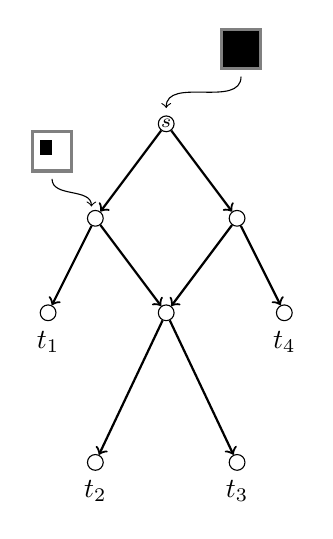
\begin{tikzpicture}
    \node[inner] (a) at (0, 0) {\scriptsize $s$};
    \node[inner] (b) at (-0.9, -1.2) {};
    \node[inner] (c) at (0.9, -1.2) {};
    \node[inner, label = below:$t_1$] (d) at (-1.5, -2.4) {};
    \node[inner] (e) at (0, -2.4) {};
    \node[inner, label = below:$t_4$] (f) at (1.5, -2.4) {};
    \node[inner, label = below:$t_2$] (g) at (-0.9, -4.3) {};
    \node[inner, label = below:$t_3$] (h) at (0.9, -4.3) {};
    
    \path (a) edge[ed] (b);
    \path (a) edge[ed] (c);
    \path (b) edge[ed] (d);
    \path (b) edge[ed] (e);
    \path (c) edge[ed] (e);
    \path (c) edge[ed] (f);
    \path (e) edge[ed] (g);
    \path (e) edge[ed] (h);
    
    \draw[very thick, gray, fill = black] (0.7, 1.2) rectangle (1.2, 0.7);
    \draw[->] (0.95, 0.6) to[out = 270, in = 90] (0, 0.2);

    \draw[very thick, gray] (-1.7, -0.1) rectangle (-1.2, -0.6);
    \fill[black] (-1.6, -0.2) rectangle (-1.45, -0.4);
    \draw[->] (-1.45, -0.7) to[out = 270, in = 90] (-0.95, -1.05);
\end{tikzpicture}

		\end{column}
	\end{columns}

\end{frame}


\begin{frame}{Circuits and protocols}

    \begin{theorem}[S 2016] 
        There is a {\color{blue}monotone} boolean circuit for function $f$ of size $S$ iff there is a
        boolean communication game of size $S$ for a relation $\Bit$ {\color{blue}$(\MBit)$} $(U =
        f^{-1}(1), V = f^{-1}(0))$.
    \end{theorem}
    
    \pause
    Proof ($\Leftarrow$):
    \begin{columns}[t]
		\begin{column}{0.65\textwidth}
            \vspace{-5mm}
            \begin{enumerate}
                \item<3-> $(H, A, B)$ is a game, $R_h = U_h \times V_h$ is a rectangle for $h \in H$.
                \item<4-> By induction we create circuits for $f_h$ such that $f_h(U_h) = 1$ and
                    $f_h(V_h) = 0$.
                \item<5-> If a leaf $h$ is marked by $i$ then $f_h = x_i$ or $f_h = \neg x_i$.
                \item<6-> For an inner vertex $h$ with children $h', h''$: $f_h = f_{h'} \land f_{h''}$
                    or $f_h = f_{h'} \lor f_{h''}$.
            \end{enumerate}
        \end{column}
        
		\begin{column}{0.35\textwidth}
            \only<5>{For all $u \in U_h$ and $v \in V_h$, $u_i \neq v_i$ $\Rightarrow$ if $u_i = 1$ and
            	$v_i = 0$ then $f_h = x_i$ else $f_h = \neg x_i$.
            }
            \only<6->{
                \vspace{-6mm}
                \begin{center}
                	\tikzstyle{end} = [thin, circle, minimum size = 0.1cm, draw, inner sep = 0.1pt]
\tikzstyle{leaf} = [thin, circle, minimum size = 0.6cm, draw, inner sep = 0.1pt, blue]
\tikzstyle{inner} = [thin, circle, minimum size = 0.2cm, draw, inner sep = 0.1pt, black]
            


\tikzstyle{ed} = [thick, ->, draw, black]

    
\begin{tikzpicture}[black]
    \draw[very thick] (0, 0) rectangle (3, 3);
	\draw[fill = gray!80!white] (0.8, 0.8) rectangle (2.1, 2.2) node[below left] {\scriptsize $R_h$};
    \only<6>{
        \draw[fill = green!20!white, opacity = 0.5, rounded corners] (0.4, 0.4) rectangle (1.4, 2.9) node[below left]
	    {\scriptsize $R_{h'}$};
	    \draw[fill = red!10!white, opacity = 0.5, rounded corners] (1.1, 0.6) rectangle (2.8, 2.5) node[below left]
	    {\scriptsize $R_{h''}$};
    }
    \only<7>{
        \draw[fill = green!20!white, opacity = 0.5, rounded corners] (0.4, 1.2) rectangle (2.8, 2.7) node[below left]
	    {\scriptsize $R_{h'}$};
	    \draw[fill = red!10!white, opacity = 0.5, rounded corners] (0.6, 1.4) rectangle (2.75, 0.5) node[above left]
	    {\scriptsize $R_{h''}$};
    }
\end{tikzpicture}
                    
	                \only<6>{
                        $f_{h'}(U_h) = f_{h''}(U_h) = 1$

                        $f_{h} = f_{h'} \land f_{h''}$
                    }
                    \only<7>{
                        $f_{h'}(V_h) = f_{h''}(V_h) = 0$

                        $f_{h} = f_{h'} \lor f_{h''}$
                    }
                \end{center}
            }
		\end{column}
	\end{columns}
\end{frame}


\begin{frame}{Communication PLS games (Razborov 1995, Kraj{\'{\i}}{\v{c}}ek 1997)}

    Difference between PLS games and \textbf{boolean} communication games:
    \begin{itemize}
        \item bounds on out-degree are removed;
        \item there is a strategy function $S$ that returns ``next'' valid vertex;
        \item the classical communication complexity of decision whether vertex is valid for $(x, y)$ and
            $S$ function is at most $k$.
    \end{itemize}

    The size of PLS game is $|H| 2^{5 t}$, where $H$ is a graph of game.

    \pause

    \begin{theorem}[S 2016]
        There is a PLS game for sets $U, V$ and some relation $N$ of size $S$ $\Leftrightarrow$ there is
        a \textbf{boolean} communication game for sets $U, V$ and the relation $N$ of size $O(S)$.
    \end{theorem}

\end{frame}


\begin{frame}{Semantic $\CP$ (Hrube{\v{s}}, 2013)}

    A proof in semantic $\CP$ for CNF formula $\phi$ is a sequence of linear inequalities with \textbf{real} coefficients
    $C_1, C_2, \dots, C_k$:
    \begin{itemize}
        \item $C_i$ is a linear inequality that encodes a clause of formula $\phi$;
        \item $C_i$ semantically followed on $\{0, 1\}$ values from $C_j, C_k$ where $j, k < i$;
        \item $C_k = (0 \ge 1)$.
    \end{itemize}

    \pause
    The size of proof is $k$. If coefficients in the proof are \textbf{integer} and bounded by some polynomial then we have a
    $\CP^*$ proof.

    \pause

    \begin{lemma}
        \begin{itemize}
            \item $\phi(x, y)$ is unsatisfiable CNF formula;
            \item $U$ is set of assignments to $x$, $V$ is a set of assignments to $y$;
            \item there is a $\CP$ \only<4>{\alert{$(\CP^*)$}} proof of $\phi$ of size $S$
        \end{itemize}
        $\Rightarrow$ there is a real \only<4>{\alert{boolean}} communication game for sets $(U, V)$ and a canonical search
        problem $\Search_{\phi}$ of size $\only<4>{\alert{poly(n)}} S$.
    \end{lemma}

\end{frame}

\begin{frame}{From $\CP$ to games}

    \begin{lemma}
        \begin{itemize}
            \item $\phi(x, y)$ is unsatisfiable CNF formula;
            \item $U$ is set of assignments to $x$, $V$ is a set of assignments to $y$;
            \item there is a $\CP$ proof of $\phi$ of size $S$
        \end{itemize}
        $\Rightarrow$ there is a real communication game for sets $(U, V)$ and a canonical search problem $\Search_{\phi}$ of
        size $S$. 
    \end{lemma}

    \pause
    Proof:
    \pause
    \begin{itemize}
        \item $H$ is a graph of the proof of $\phi$ with inverted edges;
        \pause
        \item $h \in H$, this vertex corresponds to inequalities $f(x) + \ell(y) \ge c$;
        \pause
        \item $A(h, u) = -f(u)$ and $B(h, v) = \ell(v) - c$;
        \pause    
        \item $A(h, u) > B(h, v)$ iff $f(u) + \ell(v) < c$;
        \pause
        \item root corresponds to $1 \ge 0$ $\Rightarrow$ root is valid for all inputs;
        \pause
        \item if all children of $h$ is not valid then $h$ is not valid.
    \end{itemize}
\end{frame}

\begin{frame}{Lower bound. Broken Mosquito Screen}

    Instances of Broken Mosquito Screen ($\BMS$) problem are encoding of graph with $m^2 - 2$ vertexes:
    \begin{itemize}
        \pause
        \item ``good'' instances: there is a partition of the vertexes into $m - 1$ cliques of size $m$ and one clique of size
            $m - 2$;
        \pause
		\item ``bad'' instances: there is a partition of the vertexes into $m - 1$ anticliques of size $m$ and one anticlique
            of size $m - 2$;
        \pause
        \item $G_0$ is a set of minimal good instances of the $\BMS$ problem;
        \pause
        \item $B_0$ is a set of maximal bad instances of the $\BMS$ problem.
    \end{itemize}

\end{frame}

\begin{frame}{Lower bounds}


    \begin{theorem}[S 2016]
        The size of any real communication game for sets $G_0, B_0$ and a relation $\MBit$ is at least $2^{\Omega(\sqrt{m})}$.

        If $\phi$ is a reasonable encoding of $\BMS$ problem then the size of any real communication game for sets $G_0, B_0$
        and $\Search_{\phi}$ relation is at least $2^{\Omega(\sqrt{m})}$.
    \end{theorem}

    \pause
    More powerful result:
    \begin{theorem}[Hrube{\v{s}}, Pudl{\'{a}}k 2016]
        If there is a real communication game for sets $U, V$ and $\MBit$ relation of size $S$ then there
        is a monotone real circuit that separate $U$ and $V$.
    \end{theorem}
\end{frame}


\begin{frame}{Random $\CP$}
    A $\delta$-random $\CP$ proof distribution of formula $\phi$ is a random distribution $(\pi_s,
    \Delta_s)$, where:
    \begin{itemize}
        \item $\Delta_s$ is a CNF formula;
        \item $\pi_s$ is a $\CP$ proof of $\phi \land \Delta_s$;
        \item $\forall x \in \{0, 1\}^n ~~ \Pr\limits_s[\Delta_s(x) = 1] > 1 - \delta$.
    \end{itemize}

    The size of proof $\max\limits_s \pi_s$.
    \pause

    \begin{theorem}[S 2016]
        \begin{itemize}
            \item $\phi$ is a reasonable encoding of $\BMS$;
            \item $d$ is a maximum number of clauses in formulas $\Delta_s$;
            \item $d \sqrt{\delta} \le \frac{1}{2}$
        \end{itemize}
        $\Rightarrow$ the size of $\delta$-random $\CP$ proof of $\phi$ is at least
        $2^{\Omega(\sqrt{m})}$.
    \end{theorem}
\end{frame}


\begin{frame}{$\SAT_{G}$ function (Pitassi, G{\"{o}}{\"{o}}s, 2014)}

    \begin{itemize}
        \pause
        \item Bipartite graph $G$ is fixed;
        \pause
        \item left vertices $V$ (variable nodes) and right vertices $U$ (constraint nodes);
        \pause
        \item edge $(v, u) \in E(G)$ indicates that variable $v$ is involved in constraint node $u$;
        \pause
        \item input of $\SAT_{G}$ is a truth tables for all constraints;
        \pause
        \item $\SAT_{G}$ return $1$ iff input corresponds to satisfiable $\CSP$;
        \pause
        \item $\SAT_{G}: \{0, 1\}^N \to \{0, 1\}$, where $N \le |U| \cdot 2^d$ and $d$ is the
            degree of nodes in part $U$.
    \end{itemize}

    $\SAT_{G}$ is the monotone function.

    \pause
    \begin{theorem}[S 2016]
        There is an explicit graph $G$ such that any monotone real circuit for $\SAT_{G}$ has size at
        least $2^{\Omega(N^{\frac{1}{8}})}$.
    \end{theorem}
\end{frame}

\begin{frame}{Open problems}
    \begin{enumerate}
        \pause
        \item Lower bound on boolean dag-like games for $\Search_{\phi}$ that is not based on $\MBit$.
        \pause
        \item Lower bound on boolean dag-like games for $\Search_{\phi}$ for Tseitin formulas with small
            gadgets.
        \pause
        \item Lower bound on dag-like games with new validity condition: $A(h, x) = B(h, y)$ (motivated
            by lower bounds for other proof systems).
    \end{enumerate}
\end{frame}